\documentclass{article}

\usepackage{amsmath, amssymb}
\usepackage{array}
\usepackage[a3paper, margin=1in]{geometry}
%% landscape
\usepackage{tikz}
\tikzset{
every picture/.style={very thick}
}
\usetikzlibrary{3d}

%%font
\usepackage{euler}
\usepackage[OT1]{eulervm}
\renewcommand{\rmdefault}{pplx}

\newcommand{\trans}{^\top}
\newcommand{\adj}{^{\rm adj}}
\newcommand{\cof}{^{\rm cof}}
\newcommand{\inp}[2]{\left\langle#1,#2\right\rangle}
\newcommand{\dunion}{\mathbin{\dot\cup}}
\newcommand{\bzero}{\mathbf{0}}
\newcommand{\bone}{\mathbf{1}}
\newcommand{\ba}{\mathbf{a}}
\newcommand{\bb}{\mathbf{b}}
\newcommand{\bc}{\mathbf{c}}
\newcommand{\bd}{\mathbf{d}}
\newcommand{\be}{\mathbf{e}}
\newcommand{\bh}{\mathbf{h}}
\newcommand{\bp}{\mathbf{p}}
\newcommand{\bq}{\mathbf{q}}
\newcommand{\bx}{\mathbf{x}}
\newcommand{\by}{\mathbf{y}}
\newcommand{\bz}{\mathbf{z}}
\newcommand{\bu}{\mathbf{u}}
\newcommand{\bv}{\mathbf{v}}
\newcommand{\bw}{\mathbf{w}}
\newcommand{\tr}{\operatorname{tr}}
\newcommand{\nul}{\operatorname{null}}
\newcommand{\rank}{\operatorname{rank}}
%\newcommand{\ker}{\operatorname{ker}}
\newcommand{\range}{\operatorname{range}}
\newcommand{\Col}{\operatorname{Col}}
\newcommand{\Row}{\operatorname{Row}}
\newcommand{\spec}{\operatorname{spec}}
\newcommand{\vspan}{\operatorname{span}}

\newcommand{\Var}{\operatorname{Var}}

\begin{document}
%% absolute positioning
%% \begin{tikzpicture}[remember picture, overlay]
%%   \draw ([xshift=\x]current page.south) -- ([xshift=\x]current page.north);
%% \end{tikzpicture}    

\pagenumbering{gobble}

\tikzset{
  cross/.pic={
    \draw (-2pt,-2pt) -- (2pt,2pt);
    \draw (-2pt,2pt) -- (2pt,-2pt);
  }
}

Rotational inertia of a mass of weight $m$ and of distance $R$ from the pivot point:
\[
    I = mR^2
\]

\vspace{2cm}

%% solid cylinder
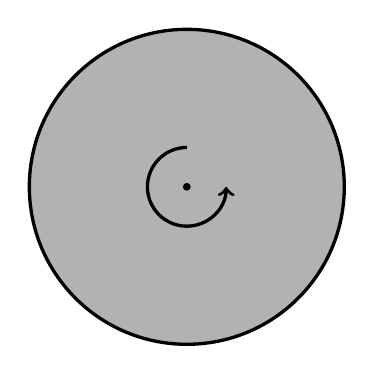
\begin{tikzpicture}
  \draw[fill=black!30] (0,0) circle (2cm);
  \node[circle, fill=black, inner sep=1pt] at (0,0) {};
  \draw[->] (90:0.5) arc (90:360:0.5);
\end{tikzpicture}
%% solid cylinder approximate
\begin{tikzpicture}
  \draw (0,0) circle (2cm);
  \node[circle, fill=black, inner sep=1pt] at (0,0) {};
  \pgfmathsetmacro{\r}{2/3}
  \pgfmathsetmacro{\twor}{4/3}
  \pic at (0,0) {cross};
  \draw (0,0) circle (\r);
  \foreach \i in {1,2,...,6} {
    \pgfmathsetmacro{\ang}{90 + 60*(\i - 1)}
    \pic at (\ang:\twor) {cross};
    \draw (\ang:\twor) circle (\r);    
  }
\end{tikzpicture}

%% hollow cylinder
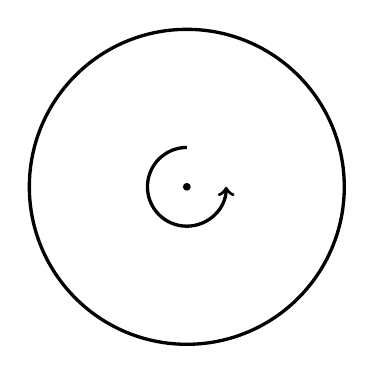
\begin{tikzpicture}
  \draw (0,0) circle (2cm);
  \node[circle, fill=black, inner sep=1pt] at (0,0) {};
  \draw[->] (90:0.5) arc (90:360:0.5);
\end{tikzpicture}
%% hollow cylinder approximate
\begin{tikzpicture}
  \draw (0,0) circle (2cm);
  \node[circle, fill=black, inner sep=1pt] at (0,0) {};
  \foreach \i in {1,2,...,6} {
    \pgfmathsetmacro{\ang}{90 + 60*(\i - 1)}
    \pgfmathsetmacro{\inang}{\ang - 28}
    \pgfmathsetmacro{\outang}{\ang + 28}
    \draw[line width=5pt, black!30] (\inang:2) arc (\inang:\outang:2);
    \pic at (\ang:2) {cross};
  }
\end{tikzpicture}

%% solid sphere
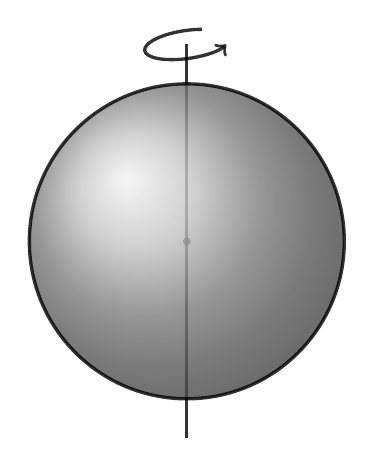
\begin{tikzpicture}[opacity=0.8]
  \draw (0,-2.5,0) -- (0,2.5,0);
  \draw[canvas is zx plane at y=2.5,->] (180:0.5) arc (180:450:0.5);
  \node[circle, fill=black, inner sep=1pt] at (0,0) {};
  \draw[ball color=black!30] (0,0) circle (2cm);
\end{tikzpicture}
%% solid sphere approximate
\begin{tikzpicture}[opacity=0.8]
  \pgfmathsetmacro{\r}{2 / (1 + sqrt(2)}
  \pgfmathsetmacro{\sqrttwor}{2 * sqrt(2) / (1 + sqrt(2)}
  \pic at (0,0,-\sqrttwor) {cross};
  \draw[canvas is xy plane at z=-\sqrttwor, ball color=black!30] (0,0) circle (\r);  
  \draw (0,-2.5,0) -- (0,2.5,0);
  \draw[canvas is zx plane at y=2.5,->] (180:0.5) arc (180:450:0.5);
  \node[circle, fill=black, inner sep=1pt] at (0,0) {};
  \draw (0,0) circle (2cm);
  \foreach \ang in {0,90,180,270} {
    \pic at (\ang:\sqrttwor) {cross};
    \draw[ball color=black!30] (\ang:\sqrttwor) circle (\r);
  }
  \pic at (0,0,\sqrttwor) {cross};
  \draw[canvas is xy plane at z=\sqrttwor, ball color=black!30] (0,0) circle (\r);
\end{tikzpicture}

%% hollow sphere
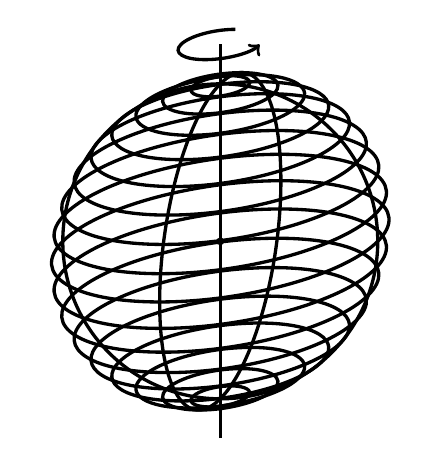
\begin{tikzpicture}
  \draw (0,-2.5,0) -- (0,2.5,0);
  \draw[canvas is zx plane at y=2.5,->] (180:0.5) arc (180:450:0.5);
  \node[circle, fill=black, inner sep=1pt] at (0,0) {};
  \draw (0,0) circle (2cm);
  \draw[canvas is yz plane at x=0] (0,0) circle (2cm);
  \foreach \phi in {-90, -80, ..., 90} {
    \pgfmathsetmacro{\cphi}{2 * cos(\phi}
    \pgfmathsetmacro{\sphi}{2 * sin(\phi}
  \draw[canvas is xz plane at y=\sphi] (0,0) circle (\cphi cm);
  }
\end{tikzpicture}
%% hollow sphere approximate
\begin{tikzpicture}[opacity=0.8]
  \pgfmathsetmacro{\r}{sqrt(2)}
  \draw[canvas is yz plane at x=-\r, ball color=black!30] (0,0) circle (\r);
  \pic at (-\r,0,0) {cross};
  \draw[canvas is zx plane at y=-\r, ball color=black!30] (0,0) circle (\r);
  \pic at (0,-\r,0) {cross};
  \draw[canvas is xy plane at z=-\r, ball color=black!30] (0,0) circle (\r);
  \pic at (0,0,-\r) {cross};
  \draw (0,-2.5,0) -- (0,2.5,0);
  \draw[canvas is zx plane at y=2.5,->] (180:0.5) arc (180:450:0.5);
  \node[circle, fill=black, inner sep=1pt] at (0,0) {};
  %% \draw (0,0) circle (2cm);
  \draw[canvas is yz plane at x=\r, ball color=black!30] (0,0) circle (\r);
  \pic at (\r,0,0) {cross};
  \draw[canvas is zx plane at y=\r, ball color=black!30] (0,0) circle (\r);
  \pic at (0,\r,0) {cross};
  \draw[canvas is xy plane at z=\r, ball color=black!30] (0,0) circle (\r);
  \pic at (0,0,\r) {cross};
  \draw (0,\r,0) -- (0,2.5,0);
\end{tikzpicture}

\begin{center}
  \begin{tabular}{|>{\centering\arraybackslash}m{2cm}|>{\centering\arraybackslash}m{2cm}|>{\centering\arraybackslash}m{2cm}|>{\centering\arraybackslash}m{2cm}|>{\centering\arraybackslash}m{2cm}|>{\centering\arraybackslash}m{3cm}|>{\centering\arraybackslash}m{7cm}|}
    \hline
    $\displaystyle x_1$ & $x_2$ & $x_3$ & $x_4$ & $x_5$ & $\displaystyle\overline{\bx} = \frac{1}{n}\sum_{i=1}^n x_i$ & $\sigma^2 = \displaystyle\frac{1}{n}\sum_{i=1}^n (x_i - \overline{\bx})^2 = \frac{1}{n}\sum_{i=1}^n x_i^2 - \overline{\bx}^2$ \\
    \hline
    ~ & ~ & ~ & ~ & ~ & ~ & ~ \\[2cm]
    \hline
    ~ & ~ & ~ & ~ & ~ & ~ & ~ \\[2cm]
    \hline
    ~ & ~ & ~ & ~ & ~ & ~ & ~ \\[2cm]
    \hline
    ~ & ~ & ~ & ~ & ~ & ~ & ~ \\[2cm]
    \hline
    ~ & ~ & ~ & ~ & ~ & ~ & ~ \\[2cm]
    \hline
    ~ & ~ & ~ & ~ & ~ & ~ & ~ \\[2cm]
    \hline
    ~ & ~ & ~ & ~ & ~ & ~ & ~ \\[2cm]
    \hline
    ~ & ~ & ~ & ~ & ~ & ~ & ~ \\[2cm]
    \hline
    ~ & ~ & ~ & ~ & ~ & ~ & ~ \\[2cm]
    \hline
    ~ & ~ & ~ & ~ & ~ & ~ & ~ \\[2cm]
    \hline
  \end{tabular}

\vspace{2cm}

average of $\sigma^2 =$
\end{center}

\end{document}





